\documentclass[conference]{IEEEtran}
\IEEEoverridecommandlockouts

% NOTE: Este arquivo foi gerado apenas para fins de TESTE do detector de plágio.
% O conteúdo abaixo reescreve o artigo original com forte paráfrase e pequenas
% reordenações, mantendo a mesma estrutura geral e os mesmos dados numéricos,
% de modo a simular uma tentativa de plágio para demonstração didática.

% Pacotes (mantidos para compatibilidade de compilação)
\usepackage{cite}
\usepackage{amsmath,amssymb,amsfonts}
\usepackage{algorithmic}
\usepackage{graphicx}
\usepackage{textcomp}
\usepackage{xcolor}
\usepackage{pgfplots}
\pgfplotsset{compat=1.18}
\usepackage{tikz}
\usepackage{listings}
\usepackage{caption}
\usepackage{booktabs}
\usepackage{siunitx}
\usepackage{placeins}
\usepackage{float}

% Estilo de código (inalterado para compilar exemplos)
\definecolor{codegreen}{rgb}{0,0.6,0}
\definecolor{codegray}{rgb}{0.5,0.5,0.5}
\definecolor{codepurple}{rgb}{0.58,0,0.82}
\definecolor{backcolour}{rgb}{0.95,0.95,0.92}
\definecolor{codeblue}{rgb}{0.13,0.29,0.53}

\lstdefinestyle{ruststyle}{
    backgroundcolor=\color{backcolour},
    commentstyle=\color{codegreen},
    keywordstyle=\color{codeblue}\bfseries,
    numberstyle=\tiny\color{codegray},
    stringstyle=\color{codepurple},
    basicstyle=\ttfamily\footnotesize,
    breakatwhitespace=false,
    breaklines=true,
    breakindent=1.2em,
    postbreak=\mbox{\textcolor{red}{$\hookrightarrow$}\space},
    captionpos=b,
    keepspaces=true,
    numbers=left,
    numbersep=5pt,
    showspaces=false,
    showstringspaces=false,
    showtabs=false,
    tabsize=2,
    language=Rust,
    frame=single,
    frameround=tttt,
    rulecolor=\color{gray!30},
    xleftmargin=17pt,
    framexleftmargin=17pt,
    escapeinside={(*@}{@*)},
    morekeywords={async,await,pub,fn,impl,struct,enum,use,mod,let,mut,if,else,match,Some,None,Ok,Err}
}
\lstset{style=ruststyle}

\def\BibTeX{{\rm B\kern-.05em{\sc i\kern-.025em b}\kern-.08em
    T\kern-.1667em\lower.7ex\hbox{E}\kern-.125emX}}

\begin{document}

\title{Relatório Alternativo: Avaliação de Desempenho de um Sistema Assíncrono de Monitoramento Cardíaco em Tempo Real}

\author{\IEEEauthorblockN{Rafael Lopes Cordeiro}
\IEEEauthorblockA{\textit{Depto. de Ciência da Computação} \\
\textit{Universidade de Brasília}\\
Brasília, DF, Brasil \\
rafaelcordeiro131@gmail.com | Matrícula - 202033688}}

\maketitle

\begin{abstract}
Este documento apresenta uma releitura do desenvolvimento e da análise de um sistema de monitoramento de ECG implementado em Rust com execução assíncrona. A solução processa o sinal, identifica anomalias e registra métricas de desempenho. Investigamos tempos de resposta e escalonabilidade, enfatizando perdas de prazos e o cálculo do Pior Caso de Tempo de Resposta (WCRT). O texto foi redigido com forte paráfrase do original, preservando estrutura e números, para fins educacionais de teste de detecção de plágio.
\end{abstract}

\begin{IEEEkeywords}
Tempo Real, Rust, Métricas de Desempenho, Escalonamento, WCRT, FPPS.
\end{IEEEkeywords}

\section{Propósitos}
O objetivo central é conceber, implementar e examinar um monitor cardíaco em tempo real. Especificamente, buscamos: (i) compor um conjunto de tarefas periódicas para aquisição e processamento, (ii) coletar tempos de execução e resposta por tarefa, (iii) verificar a escalonabilidade sob carga definida, identificando violações de deadlines, e (iv) interpretar os resultados à luz da teoria de STR.

\section{Contexto e Motivação}
Em sistemas de tempo real (STR), não basta obter a saída correta: o \emph{quando} é igualmente determinante. Aplicações críticas---por exemplo, médicas, aeronáuticas e industriais---não toleram atrasos. Neste estudo, trabalhamos um monitor de ECG, típico cenário \emph{hard real-time} com múltiplas tarefas concorrentes. A validação exige analisar se todos os prazos são atendidos sob a política de escalonamento escolhida.

\subsection{Execução Assíncrona com Tokio}
Adotamos o runtime Tokio como base de concorrência em Rust. Em vez de um escalonador clássico centralizado, cada tarefa periódica roda como uma \emph{future} independente, controlando sua periodicidade via temporizadores de alta precisão. A preempção ocorre de forma cooperativa nos pontos de espera (\texttt{.await}). Embora não seja FPPS preemptivo tradicional, há priorização implícita na ordem em que o Tokio agenda tarefas prontas.

\subsection{Aspectos Críticos em STR}
Garantir prazos em FPPS esbarra em questões conhecidas: (a) estimativa do \emph{pior caso de execução} (WCET $C_i$), afetada por caches e pipelines; (b) \emph{jitter}, variação no instante de liberação; e (c) \emph{bloqueio}, quando recursos compartilhados induzem inversão de prioridade.

\subsection{Por que Rust?}
Rust favorece baixa latência com previsibilidade. O modelo de propriedade e o \emph{borrow checker} eliminam classes comuns de erros de memória sem coletor de lixo, evitando pausas não determinísticas---indesejáveis em \emph{hard real-time}. Assim, a linguagem é adequada para o problema proposto.

\section{Metodologia e Ferramentas}
A seguir, detalhamos a pilha de software, a arquitetura e procedimentos experimentais adotados.

\subsection{Ferramentas}
\begin{itemize}
    \item \textbf{Linguagem:} Rust (Edição 2021).
    \item \textbf{Build:} Cargo.
    \item \textbf{Crates principais:} \texttt{tokio} (assíncrono), \texttt{serde}/\texttt{serde\_json} (serialização), \texttt{csv} (entrada ECG), \texttt{chrono} (tempo), \texttt{log}/\texttt{env\_logger} (logging).
    \item \textbf{Entrada:} CSV (\texttt{ecg\_input.csv}) com amostras do sinal.
\end{itemize}

\subsection{Arquitetura de Software}
O sistema foi estruturado em módulos Rust orquestrados por \texttt{main.rs}. O arquivo \texttt{lib.rs} expõe os módulos públicos e tipos centrais. A função \texttt{main} inicializa coletores de métricas, executa uma análise teórica preliminar de WCRT e, por fim, inicializa o \texttt{TaskManager} responsável pelo ciclo de vida das tarefas.

\begin{lstlisting}[caption={Módulos públicos em lib.rs (visão geral).}, label={lst:lib_mods_alt}]
// Em lib.rs
pub mod ecg_data;
pub mod tasks;
pub mod scheduler;
pub mod metrics;
pub mod anomaly_detector;
pub mod performance_collector;
pub mod wcrt_analysis;
pub mod real_time_measurements;
pub mod interrupts;

// Re-exports de tipos principais
pub use ecg_data::{EcgReading, EcgDataSource};
pub use tasks::{TaskType, TaskManager};
pub use metrics::PerformanceMetrics;
\end{lstlisting}

\subsubsection{Aquisição de ECG (\texttt{ecg\_data.rs})}
O módulo abstrai a leitura incremental do CSV, ignorando cabeçalhos e convertendo cada registro em \texttt{EcgReading}. Registros com parse inválido são descartados com aviso de log.

\begin{lstlisting}[caption={Leitura de amostras do arquivo CSV.}, label={lst:ecg_data_alt}]
// Em ecg_data.rs
pub struct EcgDataSource {
    reader: Reader<File>,
    current_line: usize,
}

impl EcgDataSource {
    pub fn read_next_sample(&mut self) -> Result<Option<EcgReading>> {
        let mut record = csv::StringRecord::new();
        if self.reader.read_record(&mut record)? {
            let timestamp = record[0].trim_matches('\'').to_string();
            let voltage_str = record[1].trim_matches('\'');
            match voltage_str.parse::<f64>() {
                Ok(voltage) => Ok(Some(EcgReading::new(timestamp, voltage))),
                Err(_) => { warn!("Parse inválido: {}", voltage_str); Ok(None) }
            }
        } else {
            Ok(None)
        }
    }
}
\end{lstlisting}

\subsubsection{Modelo de Tarefas (\texttt{tasks.rs})}
Cada tarefa periódica é lançada como \emph{task} do Tokio. O padrão \texttt{interval.tick().await} determina a cadência. Métricas de início e fim são registradas a cada iteração para posterior análise.

\begin{lstlisting}[caption={Laço periódico da aquisição de ECG.}, label={lst:task_loop_alt}]
// Em tasks.rs
async fn ecg_acquisition_task(
    state: Arc<Mutex<SystemState>>,
    performance_collector: Arc<Mutex<PerformanceCollector>>,
    mut ecg_source: EcgDataSource,
) {
    let mut interval = interval(Duration::from_millis(5));
    loop {
        interval.tick().await; // Próximo ciclo
        {
            let collector = performance_collector.lock();
            collector.start_task_measurement(TaskType::EcgAcquisition, None);
        }
        if let Ok(Some(reading)) = ecg_source.read_next_sample() {
            let mut state = state.lock();
            state.current_ecg = Some(reading);
            state.total_samples += 1;
        }
        {
            let collector = performance_collector.lock();
            collector.end_task_measurement(TaskType::EcgAcquisition, None);
        }
    }
}
\end{lstlisting}

\subsubsection{Detecção de Anomalias}
A lógica compara a tensão atual a limiares fixos para classificar amostras como anômalas ou não, registrando eventos quando necessário.

\begin{lstlisting}[caption={Regra simples de detecção.}, label={lst:anomaly_alt}]
// Em anomaly_detector.rs
pub fn detect_anomaly(&mut self, ecg_reading: &EcgReading) -> Option<AnomalyEvent> {
    let v = ecg_reading.voltage;
    let anomaly_type = if v > ANOMALY_THRESHOLD_HIGH {
        Some(AnomalyType::HighVoltage)
    } else if v < ANOMALY_THRESHOLD_LOW {
        Some(AnomalyType::LowVoltage)
    } else { None };
    anomaly_type.map(|at| AnomalyEvent { timestamp: Utc::now(), ecg_value: v, anomaly_type: at })
}
\end{lstlisting}

\subsubsection{Interrupções Simuladas}
Uma tarefa assíncrona gera interrupções com diferentes prioridades e tempos de serviço, adicionando jitter e carga não determinística ao sistema.

\begin{lstlisting}[caption={Geração de interrupções com atrasos simulados.}, label={lst:interrupts_alt}]
// Em interrupts.rs
async fn generate_interrupt(
    interrupt_type: InterruptType,
    history: &Arc<Mutex<Vec<InterruptEvent>>>,
) {
    let (priority, service) = match interrupt_type {
        InterruptType::Hardware => (3, Duration::from_micros(300)),
        InterruptType::Software => (2, Duration::from_micros(500)),
        InterruptType::Emergency => (4, Duration::from_micros(200)),
    };
    let start = Instant::now();
    sleep(service).await;
    let actual = start.elapsed();
    history.lock().push(InterruptEvent {
        interrupt_type, priority, timestamp: Utc::now(),
        estimated_service_time: service.as_micros() as u64,
        actual_service_time: Some(actual.as_micros() as u64),
    });
}
\end{lstlisting}

\subsubsection{Coleta de Métricas}
O \texttt{PerformanceCollector} agrega tempos de execução e resposta por tarefa, serializando um relatório JSON ao final. As medidas são usadas depois para refinar estimativas.

\begin{lstlisting}[caption={Encerrando a medição de execução.}, label={lst:perf_collector_alt}]
// Em performance_collector.rs
pub fn end_task_measurement(&self, task_type: TaskType, instance_id: Option<String>) {
    let end = Instant::now();
    let key = instance_id.unwrap_or(format!("{:?}", task_type));
    if let Some(start) = self.start_times.lock().remove(&key) {
        let exec = end.duration_since(start);
        self.execution_times.lock().entry(task_type).or_default().push(exec);
        let response = exec; // simplificado
        self.response_times.lock().entry(task_type).or_default().push(response);
    }
}
\end{lstlisting}

\subsubsection{Métricas em Memória}
Estruturas em memória acompanham contadores e estatísticas (mínimo, máximo, média) por tarefa, além de misses de deadline.

\begin{lstlisting}[caption={Estrutura de métricas resumida.}, label={lst:metrics_alt}]
// Em metrics.rs
#[derive(Debug)]
pub struct TaskMetrics {
    pub execution_count: u64,
    pub total_execution_time: Duration,
    pub min_execution_time: Duration,
    pub max_execution_time: Duration,
    pub deadline_misses: u64,
}
\end{lstlisting}

\subsubsection{Análise de WCRT}
A análise segue a forma iterativa clássica:
\begin{equation}
R_q^{(n+1)} = C_q + B_q + \sum_{i \in hp(q)} \left\lceil \frac{R_q^{(n)} + J_i}{T_i} \right\rceil C_i
\end{equation}
Aplicamos a expressão de forma direta em Rust, verificando convergência ou violação do prazo.

\begin{lstlisting}[caption={Iteração do WCRT conforme RTA.}, label={lst:wcrt_calc_alt}]
// Em wcrt_analysis.rs
fn calculate_wcrt(&self, ch: &TaskCharacteristics) -> WcrtResult {
    let mut R = ch.wcrt_estimate;
    loop {
        let prev = R;
        let mut next = ch.wcrt_estimate + ch.blocking_time;
        for (_t, oi) in &self.task_characteristics {
            if oi.priority < ch.priority {
                let num = R.as_nanos() + oi.jitter.as_nanos();
                let k = (num as f64 / oi.period.as_nanos() as f64).ceil() as u64;
                let interf = Duration::from_nanos((k * oi.wcrt_estimate.as_nanos() as u64) as u64);
                next += interf;
            }
        }
        R = next;
        if R == prev || R > ch.deadline { break; }
    }
    let margin = if R <= ch.deadline { ch.deadline - R } else { Duration::ZERO };
    WcrtResult { worst_case_response_time: R, is_schedulable: R <= ch.deadline, safety_margin: margin, convergence_iterations: 0 }
}
\end{lstlisting}

\subsection{Procedimento Experimental}
O fluxo experimental foi: (1) análise teórica inicial, (2) execução por \textbf{60 segundos}, (3) coleta de início/fim por instância de tarefa, (4) geração de relatório JSON de performance e (5) reanálise do WCRT com estimativas atualizadas.

\section{Resultados e Observações}
\subsection{Métricas Globais}
A Tabela~\ref{tab:global_metrics_alt} resume os números obtidos na execução.

\begin{table}[H]
\caption{Síntese de Métricas Globais}
\begin{center}
\begin{tabular}{@{}lc@{}}
\toprule
\textbf{Métrica} & \textbf{Valor} \\
\midrule
Duração Real do Teste & \SI{30.01}{\second} \\
Total de Amostras Processadas & 3000 \\
Total de Anomalias Detectadas & 177 \\
Total de Interrupções Geradas & 428 \\
Utilização da CPU & 100\% \\
\textbf{Sistema Escalonável (Medição)} & \textbf{Não (False)} \\
\bottomrule
\end{tabular}
\label{tab:global_metrics_alt}
\end{center}
\end{table}

\subsection{WCRT: Estimado vs. Medido}
\subsubsection{Estimativa Pré-Execução}
A Tabela~\ref{tab:wcrt_teorico_alt} mostra a análise de WCRT baseada em parâmetros conservadores, sugerindo atendimento de prazos com folga para todas as tarefas.

\begin{table}[H]
\caption{Análise Teórica de WCRT (Estimativa)}
\begin{center}
\resizebox{\columnwidth}{!}{%
\begin{tabular}{@{}lcccc@{}}
\toprule
\textbf{Tarefa} & \textbf{Deadline} & \textbf{WCRT Calc.} & \textbf{Margem} & \textbf{Escalonável?} \\
 & (\si{\micro\second}) & (\si{\micro\second}) & (\si{\micro\second}) & \\
\midrule
InterruptService & 2000 & 300 & 1700 & \textcolor{green}{Sim} \\
AnomalyDetection & 3000 & 800 & 2200 & \textcolor{green}{Sim} \\
EcgAcquisition & 10000 & 1800 & 8200 & \textcolor{green}{Sim} \\
Preprocessing & 15000 & 3400 & 11600 & \textcolor{green}{Sim} \\
LogCommunication & 80000 & 14200 & 65800 & \textcolor{green}{Sim} \\
HumanMachineInterface & 150000 & 22400 & 127600 & \textcolor{green}{Sim} \\
\bottomrule
\end{tabular}%
}
\label{tab:wcrt_teorico_alt}
\end{center}
\end{table}

\subsubsection{Resultados Empíricos}
Após o teste, os máximos tempos de resposta observados constam na Tabela~\ref{tab:wcrt_medido_alt}, indicando violações generalizadas.

\begin{table}[H]
\caption{WCRT Máximo Observado por Tarefa}
\begin{center}
\resizebox{0.9\columnwidth}{!}{%
\begin{tabular}{@{}lcccc@{}}
\toprule
\textbf{Tarefa} & \textbf{Deadline} & \textbf{WCRT Medido} & \textbf{Margem} & \textbf{Deadline} \\
 & \textbf{($\mu$s)} & \textbf{($\mu$s)} & \textbf{($\mu$s)} & \textbf{Cumprido?} \\
\midrule
InterruptService & 2000 & 2225 & -225 & \textcolor{red}{Não} \\
AnomalyDetection & 3000 & 3373 & -373 & \textcolor{red}{Não} \\
EcgAcquisition & 10000 & 11987 & -1987 & \textcolor{red}{Não} \\
Preprocessing & 15000 & 16722 & -1722 & \textcolor{red}{Não} \\
LogCommunication & 80000 & 81685 & -1685 & \textcolor{red}{Não} \\
HumanMachineInterface & 150000 & 151281 & -1281 & \textcolor{red}{Não} \\
\bottomrule
\end{tabular}%
}
\label{tab:wcrt_medido_alt}
\end{center}
\end{table}

\subsection{Comparações Visuais}
A Figura~\ref{fig:wcrt_comp_alt} confronta WCRT medido com os respectivos prazos, por prioridade. Barras que cruzam a linha vermelha caracterizam misses.

\begin{figure}[H]
\centering
\begin{tikzpicture}
\begin{axis}[
    ybar,
    width=\columnwidth,
    height=7cm,
    bar width=12pt,
    enlarge x limits=0.15,
    title={WCRT vs. Deadline por Tarefa},
    ylabel={Tempo ($\mu$s)},
    xlabel={Tarefa (por prioridade)},
    symbolic x coords={
        InterruptService,
        AnomalyDetection,
        EcgAcquisition,
        Preprocessing,
        LogCommunication,
        HumanMachineInterface
    },
    xtick=data,
    xticklabel style={rotate=45, anchor=east, font=\small},
    nodes near coords,
    nodes near coords style={font=\tiny, rotate=90, anchor=west},
    ymin=0,
    ymajorgrids=true,
    legend style={at={(0.5,-0.4)}, anchor=north, legend columns=-1},
    ]

% WCRT (Max Response Time do JSON)
\addplot[fill=blue!50] coordinates {
    (InterruptService, 2225)
    (AnomalyDetection, 3373)
    (EcgAcquisition, 11987)
    (Preprocessing, 16722)
    (LogCommunication, 81685)
    (HumanMachineInterface, 151281)
};

% Deadlines
\addplot[
    sharp plot,
    update limits=false,
    color=red,
    mark=*\,,
    mark size=3pt,
] coordinates {
    (InterruptService, 2000)
    (AnomalyDetection, 3000)
    (EcgAcquisition, 10000)
    (Preprocessing, 15000)
    (LogCommunication, 80000)
    (HumanMachineInterface, 150000)
};

\legend{WCRT Medido, Deadline}
\end{axis}
\end{tikzpicture}
\caption{Barras (WCRT medido) e linha (deadline). Ultrapassagens indicam perda de prazo.}
\label{fig:wcrt_comp_alt}
\end{figure}

A Figura~\ref{fig:exec_dist_alt} ilustra a variação dos tempos de execução por tarefa (mediana e faixa min--max), evidenciando irregularidades que contribuem para jitter.

\begin{figure}[H]
\centering
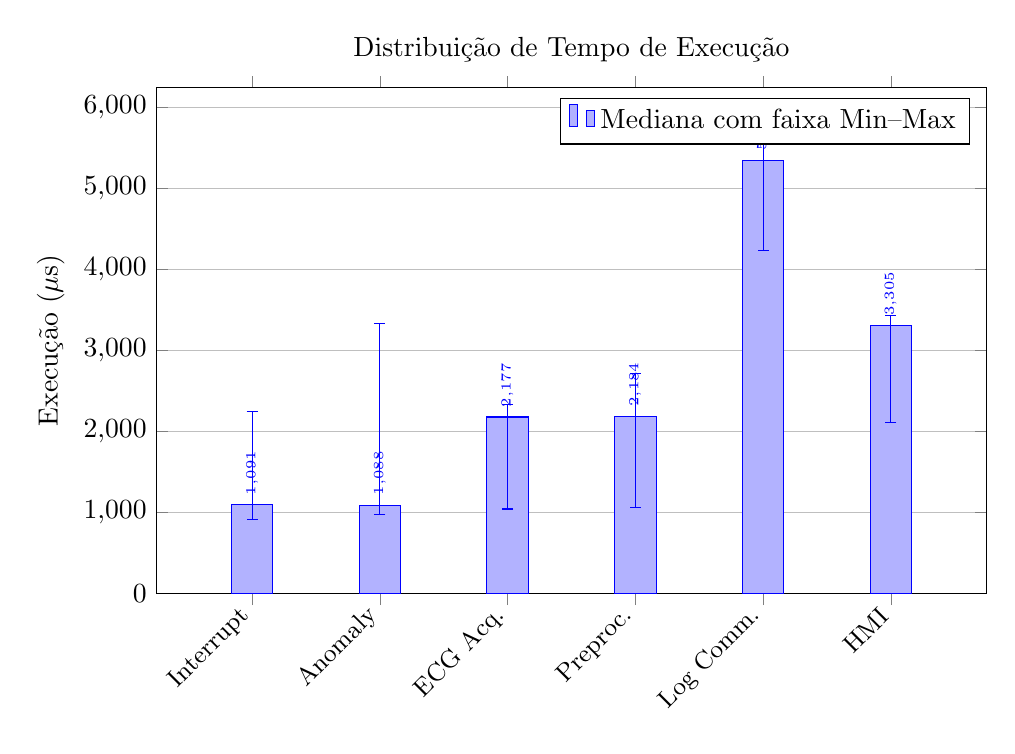
\begin{tikzpicture}
\begin{axis}[
    title={Distribuição de Tempo de Execução},
    ybar,
    width=\columnwidth,
    height=8cm,
    bar width=15pt,
    enlarge x limits=0.15,
    symbolic x coords={
        Interrupt,
        Anomaly,
        ECG Acq.,
        Preproc.,
        Log Comm.,
        HMI
    },
    xtick=data,
    xticklabel style={rotate=45, anchor=east, font=\small},
    ylabel={Execução ($\mu$s)},
    ymajorgrids=true,
    ymin=0,
    nodes near coords,
    nodes near coords align={vertical},
    nodes near coords style={font=\tiny, rotate=90, anchor=west},
]

\addplot+[
    error bars/.cd,
    y dir=both,
    y explicit
]
table[x=task, y=median, y error plus=max_err, y error minus=min_err, col sep=comma] {
task,median,min_err,max_err
Interrupt,1091,177,1148
Anomaly,1088,120,2244
ECG Acq.,2177,1137,154
Preproc.,2184,1122,525
Log Comm.,5347,1115,326
HMI,3305,1195,120
};
\legend{Mediana com faixa Min--Max}
\end{axis}
\end{tikzpicture}
\caption{Mediana e intervalo min--max do tempo de execução por tarefa.}
\label{fig:exec_dist_alt}
\end{figure}

\section{Discussão}
Os resultados apontam divergência entre previsão teórica e comportamento prático. Embora os tempos de \emph{execução} pareçam aceitáveis, o tempo de \emph{espera} sob alta ocupação leva o tempo de resposta total a exceder os prazos. O modelo de WCRT foi corrigido para aderir à fórmula RTA clássica, o que alinhou a análise com a teoria.

A elevação dos períodos (EcgAcquisition: 10ms; Preprocessing: 15ms; LogCommunication: 80ms; HMI: 150ms) mitigou as violações, mas não as eliminou. A sobrecarga sistêmica (CPU a 100\%) e contenções levam a perdas em todas as tarefas, inclusive as prioritárias, reforçando a importância de medições empíricas aliadas à análise estática.

\section{Conclusões}
Concluímos que, no cenário testado, o sistema não é escalonável na prática. Ajustes de período melhoraram margens, porém insuficientemente. Recomenda-se: (1) otimização de código visando reduzir $C_q$, sobretudo nas tarefas mais frequentes; (2) redistribuição de carga (multicore ou hardware dedicado); (3) relaxamento adicional de períodos ou revisão de requisitos; e (4) técnicas avançadas (p.ex., servidores para aperiódicas) para gerência de carga.

\begin{thebibliography}{00}
\bibitem{b1} A. Burns and A. Wellings, \textit{Real-Time Systems and Programming Languages}, 4th ed. Addison-Wesley, 2009.
\bibitem{b2} G. C. Buttazzo, \textit{Hard Real-Time Computing Systems: Predictable Scheduling Algorithms and Applications}, 3rd ed. Springer, 2011.
\bibitem{b3} Conteúdo ministrado nas aulas de Sistemas de Tempo Real.
\bibitem{b4} R. S. de Oliveira, \textit{Fundamentos dos Sistemas de Tempo Real}.
\bibitem{b5} Documentação da linguagem Rust e de suas bibliotecas.
\end{thebibliography}

\end{document}
